\section{Kolejność taśmociągów}

Trzy napędy nie są niezależnymi silnikami. Stoją w jednej linii, więc załączenie kolejnego odcinka powinno zależeć od tego, czy odcinek, który ma odebrać albo podać materiał, naprawdę pracuje.

\subsection{Bieg od początku linii}

W czwartej wersji, na szczeblach napędu 2 i napędu 3, dołożyliśmy styki wyjść poprzedników. Q2 może się załączyć dopiero wtedy, gdy jest już Q1, a Q3 dopiero wtedy, gdy jest Q2. Sam pierwszy napęd pozostaje warunkiem koniecznym dla dwóch pozostałych: jeśli Q1 odpadnie (STOP, zanik M1 albo awaria na I3), szereg za nim też traci sygnał. Timery nadal odmierzają odstępy, ale czas nie wystarcza --- musi być jeszcze potwierdzenie pracy poprzedniego odcinka.

% \begin{figure}[H]
%     \centering
%     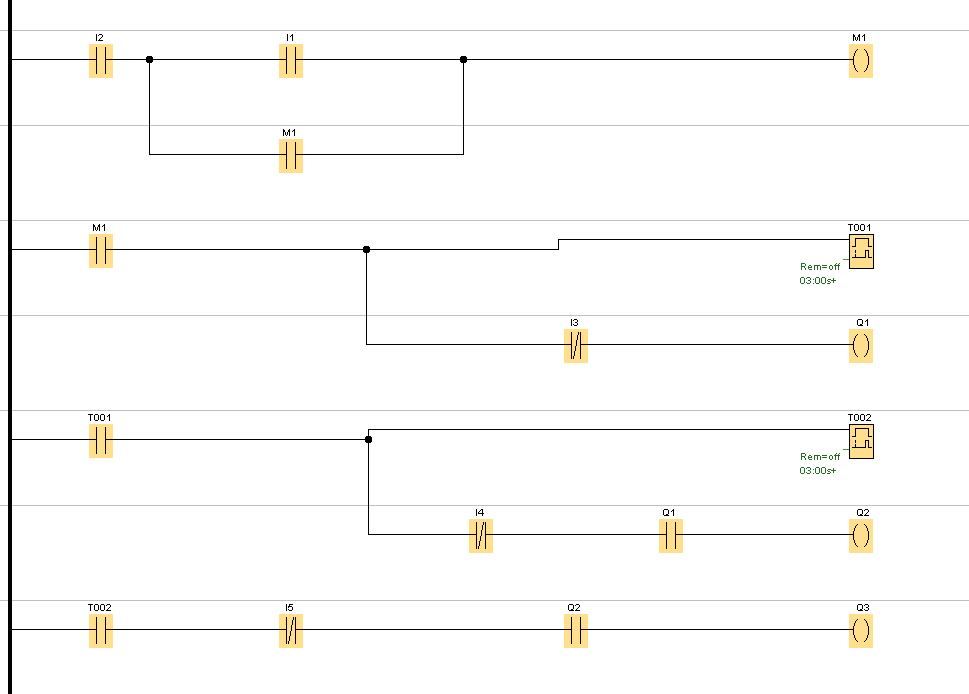
\includegraphics[width=0.92\textwidth]{rys/iteracja4.png}
%     \caption{Iteracja 4 --- Q2 zależne od Q1, Q3 zależne od Q2}
%     \label{fig:iter4}
% \end{figure}

\subsection{Bieg od końca linii}

Przy taśmociągach częściej rozruch prowadzi się od końca ciągu, żeby materiał miał gdzie spadać i nie piętrzył się na nieruchomym odcinku. Piąta iteracja jest tą samą drabinką, ze zmienioną kolejnością:

\begin{itemize}
    \item na szczeblu, który dotąd stawiał Q1, jest Q3, a informacja o awarii pochodzi z I5,
    \item załączenie środkowego napędu zależy od Q3, a nie od Q1,
    \item ostatni szczebel wystawia Q1 i pilnuje awarii z toru pierwszego napędu.
\end{itemize}

Efekt jest odwrotny niż w iteracji 4: najpierw rusza końcowy odcinek, potem środkowy, na końcu pierwszy, każdy z opóźnieniem i każdy pod warunkiem, że poprzedni w tej kolejności już pracuje. Awaria nadal zdejmuje swój napęd, a STOP gasi marker i całą kaskadę.

% \begin{figure}[H]
%     \centering
%     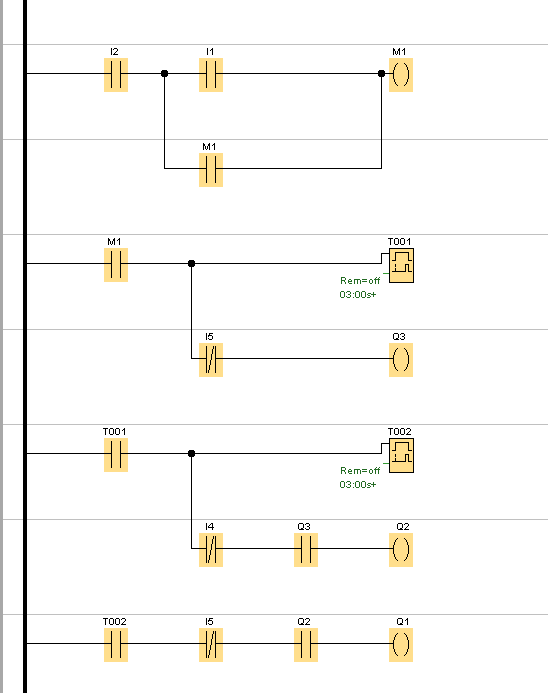
\includegraphics[width=0.92\textwidth]{rys/iteracja5.png}
%     \caption{Iteracja 5 --- rozruch od końca linii}
%     \label{fig:iter5}
% \end{figure}

% \begin{figure}[H]
%     \centering
%     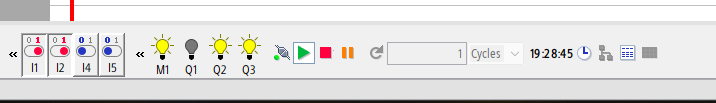
\includegraphics[width=0.85\textwidth]{rys/symulacja.png}
%     \caption{Symulacja końcowej wersji w LOGO! Soft Comfort}
%     \label{fig:symulacja}
% \end{figure}

% \begin{figure}[H]
%     \centering
%     \includegraphics[width=0.85\textwidth]{rys/sterownik.png}
%     \caption{Ten sam program uruchomiony na sterowniku LOGO!}
%     \label{fig:sterownik}
% \end{figure}

\subsection{Co sprawdziliśmy}

Końcową wersję (iteracja 5) przeszliśmy w symulatorze, a potem na sterowniku. Zachowanie, którego oczekiwaliśmy, i to, co wyszło, jest w tabeli~\ref{tab:testy}.

\begin{table}[h]
    \centering
    \caption{Testy końcowej wersji programu}
    \label{tab:testy}
    \begin{tabular}{|c|p{5.2cm}|p{5.6cm}|c|}
        \hline
        \textbf{Nr} & \textbf{Warunek} & \textbf{Oczekiwany skutek} & \textbf{Wynik} \\
        \hline
        1 & impuls START na I1 & M1 zostaje, Q3 po chwili, potem Q2 i Q1 & OK \\
        \hline
        2 & puszczenie START & napędy dalej pracują dzięki M1 & OK \\
        \hline
        3 & STOP na I2 & M1 i wszystkie Q gasną, timery wracają do zera & OK \\
        \hline
        4 & powrót zasilania bez START & układ stoi & OK \\
        \hline
        5 & awaria na I5 przy pracy & odpada napęd 3 i kaskada za nim & OK \\
        \hline
        6 & Q3 zgaszone & Q2 i Q1 nie wstają same & OK \\
        \hline
    \end{tabular}
\end{table}

Różnica między symulacją a sterownikiem nie dotyczyła samej drabinki. W symulatorze wejścia przełączaliśmy myszką i czasy były idealne. Na LOGO! ten sam program czyta prawdziwe przyciski, więc liczy się filtr wejść i to, czy styk awaryjny jest zwarty w stanie normalnym. Kolejność szczebli i nastawy T1 oraz T2 przenieśliśmy bez zmian.
